\chapter{Risultati Sperimentali}
\captionsetup[table]{name=Tabella}
I dati analizzati comprendono tutte le transazioni Bitcoin dal \textbf{3 Gennaio 2009} al \textbf{10 Agosto 2017}.

Come spiegato precedentemente il primo obiettivo è quello di presentare statistiche generali sull'uso del dust, mostrare gli effetti del dust sulla de-anonimizzazione di address e, infine, descrivere pattern che potrebbero rappresentare dei Dust Attack.

\section{Filtraggio transazioni}
Il primo compito è stato il filtraggio di tutte le transazioni dust, ovvero tutte quelle transazioni che comprendono tra gli input e/o tra gli output un importo minore di 546 satoshi, valore di riferimento del dust.
\begin{figure}[H]
\begin{mdframed}
 infos:inputs:118890,\green{99},2;118902,9987098901,2 \checkmark\\
 infos:21482214,984902,114569039,1;21482868,\green{1},73028796,240:outputs \checkmark\\
 infos:118925,9963398109,121409,0:118926,9962398010,2 \red{x}
\end{mdframed}
\caption{Esempi di transazioni accettate o rifiutate}
\label{tx_dust}
\end{figure}
\Floatbarrier
La figura \ref{tx_dust} mostra due esempi di transazioni dust e uno di transazione non-dust, le prime due transazioni vengono considerate nelle analisi successive perché contengono importi dust, mentre la terza viene scartata. 

La prima infatti contiene, tra gli output, un importo di 99 satoshi, la seconda invece contiene un importo di 1 satoshi tra gli input. L'ultima transazione invece è stata scartata proprio perché tutti gli importi sono maggiori o uguali a 546 satoshi. Le transazioni non-dust di questo tipo sono state ignorate poichè le analisi vertono sulla generazione e sul consumo del dust e sulla de-anonimizzazione causata da questi importi.

Le transazioni totali sono 245 410 083 mentre le transazioni che generano o consumano dust sono  2 114 335. Questo significa che il dust è usato solo nello 0.8\% delle transazioni totali. Inoltre, come confermato da \cite{dustAnalisi}, 1 705 560 creano dust mentre solo 429 544 lo consumano. Siccome la somma delle transazioni che consumano dust e delle transazioni che generano il dust è superiore al totale delle transazioni possiamo dedurre che ci siano transazioni in cui il dust è presente sia negli input che negli output.

Il passaggio successivo è stato il filtraggio delle transazioni generate da Satoshi Dice poichè non riteniamo siano parte di Dust Attack. Satoshi Dice, come spiegato in precedenza, è un noto servizio di gambling nato nell'Aprile 2012. Questo servizio utilizza il dust per comunicare ai giocatori l'esito perdente della loro scommessa. Data la notorietà del servizio, risulta molto poco probabile che l'intento sia quello di un Dust Attack, inoltre le analisi vogliono mostrare il comportamento degli utenti nei confronti del dust proveniente da address sconosciuti. Non solo gli address di Satoshi Dice sono noti proprio perché il servizio stesso li ha resi pubblici, ma l'indirizzo di ricezione del dust dello scommettitore è lo stesso con cui la scommessa viene piazzata, e quindi non scelto discrezionalmente dal servizio.

Le transazioni generate da Satoshi Dice sono 1 465 295, ovvero il 69\% delle transazioni dust. Questo risultato, oltre a dimostrare la popolarità del servizio, permette di concentrare le future analisi sul rimanente 31\%(649 040) delle transazioni.

\section{Analisi del dust}
Una volta ottenute tutte e sole le transazioni di interesse sono stati realizzati gli istogrammi mostrati in figura \ref{fig:dust_distribuzione}. L'istogramma, mostrato nella parte sinistra della figura \ref{fig:dust_distribuzione}, mostra la distribuzione del numero di input dust, quello a destra invece la distribuzione del numero di output dust. In entrambi i grafici non sono state contate le transazioni con 0 importi dust. La prima colonna quindi rappresenta, in entrambi gli istogrammi, l'intervallo [1, 50].
\begin{figure}[h!]
    \centering
    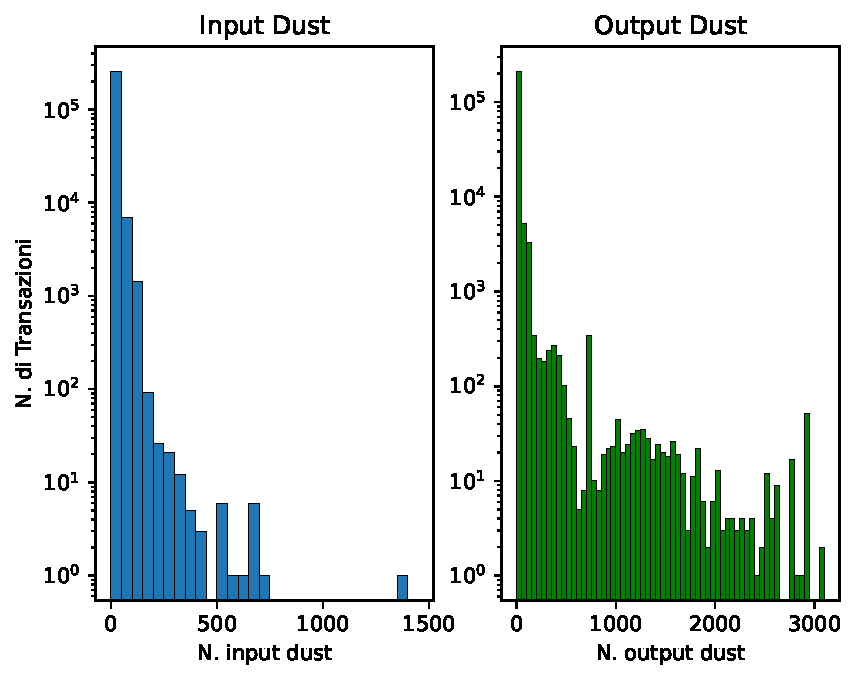
\includegraphics[scale=0.9]{Grafici/distribuzione_dust.pdf}
    \caption{Distribuzione numero input dust(sinistra) e output dust(destra). Intervalli di ampiezza pari a 50 con primo intervallo [1, 50]. Si noti la scala logaritmica sull'asse delle ordinate}
    \label{fig:dust_distribuzione}
\end{figure}
\FloatBarrier 
Entrambi gli istogrammi mostrano come siano molto frequenti le transazioni presenti nel primo intervallo di ampiezza [1, 50]. Nel primo grafico notiamo anche che le transazioni con un elevato numero di input dust risultino poco frequenti. Al contrario del primo grafico, il secondo mostra come siano presenti tante transazioni che generano un elevato numero di output dust. Dall'analisi di questi due grafici inoltre possiamo già intuire che diversi output dust generati non vengano successivamente spesi.

Manualmente ispezionando alcune delle numerose transazioni con un numero basso di input o output, abbiamo intuito di poter introdurre un livello di filtraggio ulteriore. In tutte le analisi successive viene infatti considerato solo il dust generato con script diverso da OP\_RETURN. Questa scelta è motivata dal fatto che gli output con questo script non possono essere spesi, questa tipologia di dust quindi non può avere effetti sulla de-anonimizzazione. E quindi, chi lo sta generando sicuramente non sta attuando un Dust Attack. In totale sono presenti 18 357 output dust con questo script, di cui il 97.5\% ha come importo 1 satoshi.

Il grafico \ref{fig:dust_created} mostra quindi la distribuzione nel tempo degli output dust rimanenti (cioè quelli potenzialmente spendibili).
\begin{figure}[h!]
    \centering
    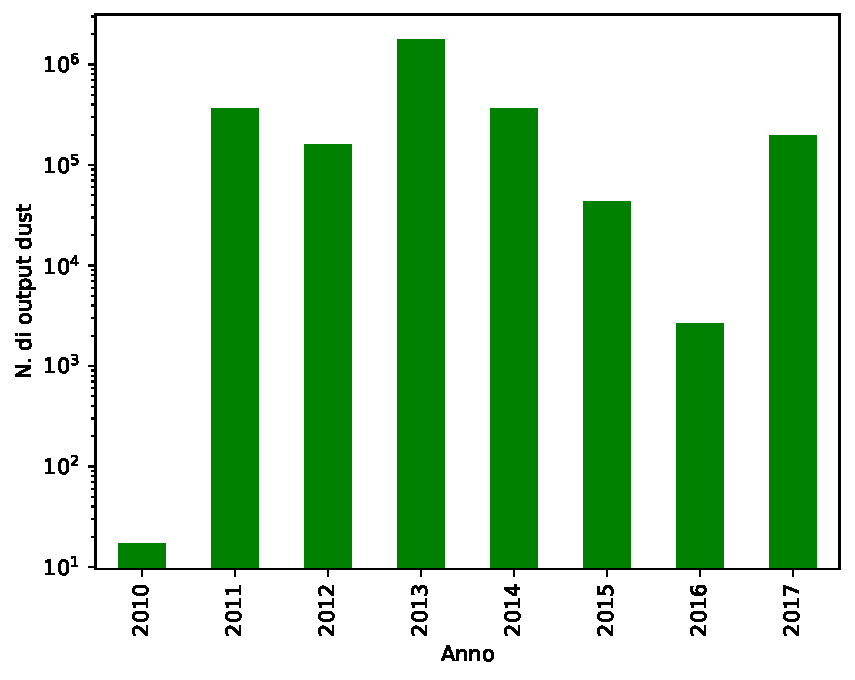
\includegraphics[scale=0.9]{Grafici/dust_created_year.pdf}
    \caption{Distribuzione delle date di creazione di output dust (filtrati) nel tempo}
    \label{fig:dust_created}
\end{figure}
\FloatBarrier 

Dal grafico è possibile notare che a partire dal 2010 sono comparsi i primi output dust, anche se in quantità molto ridotta. Possiamo osservare un rapido aumento tra il 2010 e il 2011. Solo nel mese di luglio dell'anno 2011 infatti sono stati generati più di 27 000 output dust.

Il picco della generazione di dust è presente nel 2013, dove sono stati trovati pattern interessanti di transazioni legate ``a catena". Nel paragrafo successivo verranno approfonditi questi schemi. Dopo il picco del 2013 osserviamo una costante diminuzione negli anni fino al 2017 dove si assiste ad un nuovo incremento. Bisogna però specificare che circa il 95\% del dust generato nel 2017 proviene da due address: $1Enjoy1C4bYBr3tN4sMKxvvJDqG8NkdR4Z$ e $1SochiWwFFySPjQoi2biVftXn8NRPCSQC$.

Questi due noti address sono comparsi per la prima volta nel 2014, in concomitanza con le olimpiadi di Sochi in Russia, generando transazioni con circa 750 output di 1 satoshi ciascuno. È importante notare come, nonostante il caos causato in vari forum Bitcoin, la tempesta di spam del 2014 ``Enjoy Sochi" abbia lasciato un'impronta relativamente piccola sulla blockchain. Solo 65 transazioni(48 750 output dust) sono state confermate in quell'anno.

L'aspetto singolare di questo fenomeno è che abbiamo visto dei suoi echi tornare negli anni successivi. Nel 2015 infatti sono state confermate 23 transazioni(17 250 output dust) mentre nel 2017 sono presenti 255 transazioni(189 495 output dust) generate da questi vanity address. Sebbene sia possibile che siano state eseguite dalla stessa entità, che spendeva importi da quegli address anche nel 2018, è anche possibile che queste transazioni fossero state generate nel 2014 e confermate solo nel 2015 e nel 2017. In questi tre anni il fenomeno ``Enjoy Sochi" ha generato un totale di 343 transazioni per un totale di output dust intorno ai 255 000.

In generale sono stati generati 2 893 877 output dust filtrati (ossia non imputabili a Satoshi Dice e con script diverso da OP\_RETURN), e circa il 48.5\% è stato speso. Quindi la quantità di dust non speso (51.5\%) è simile a quello speso. 

La tabella \ref{tab:dust_spent_unspent} mostra il rapporto in percentuale negli anni del numero di output dust generati e il numero di output dust spesi e non-spesi, non necessariamente il dust è stato speso nello stesso anno in cui è stato generato ma può essere stato speso anche in anni successivi. Il 2009 non è stato considerato perché non è stato generato alcun output dust in quell'anno. La superiorità del dust non-speso rispetto al dust speso è presente soprattutto negli anni 2011 e 2017, anche se parte del dust del 2017 potrebbe essere stato speso successivamente al 10 Agosto 2017, data dell'ultima transazione del dataset. Il 2010, nonostante il dust non-speso sia l'83\%, non è molto rilevante poichè sono stati generati solo 14 output dust in totale. 
\begin{table}[H]
    \centering
    \begin{tabular}{|c|c|c|c|c|c|c|c|c|}
        \hline
           categoria/anno   & 2010 & 2011 & 2012 & 2013 & 2014 & 2015 & 2016 & 2017\\
        \hline 
         speso &  17\% & 0,2\% & 54\% & 44\% & 76\% & 94,6\% & 95,6\% & 10\% \\
         \hline
         non-speso & 83\% & 99,8\% & 46\% & 56\% & 24\% & 5,4\% & 4,4\% & 90\%  \\
         \hline
    \end{tabular}
    \caption{Dust Speso e Non-Speso negli anni}
    \label{tab:dust_spent_unspent}
\end{table}
\section{Classificazione del dust}
Come descritto in sezione~\ref{algoritmii} gli output dust sono stati suddivisi in quattro categorie:
\begin{enumerate}
    \item \textbf{Successo}: dust speso in transazioni che presentano almeno due address diversi di input, in queste transazioni la fee è diversa dall'importo totale di input;
    \item \textbf{Fallimento}: dust speso in transazioni con un solo address di input, anche se ripetuto più volte;
    \item \textbf{Speciale}: dust speso in possibili transazioni di ``dust collecting", transazioni la cui fee è uguale all'importo totale di input;
    \item \textbf{Non speso}.
\end{enumerate}

I termini ``Successo" e ``Fallimento" si riferiscono alla possibilità di collegare gli address di input una volta che il dust è stato speso. Nonostante il ``dust-collecting" rappresenti un caso di de-anonimizzazione fallita, poichè gli address di input potrebbero appartenere ad utenti diversi, questa situazione viene separata dalla categoria ``Fallimento" per mostrare se e quanto questa tecnica sia stata utilizzata.

Il grafico \ref{fig:dust_year} mostra la distribuzione delle categorie nel corso degli anni.
\begin{figure}[h!]
    \centering
    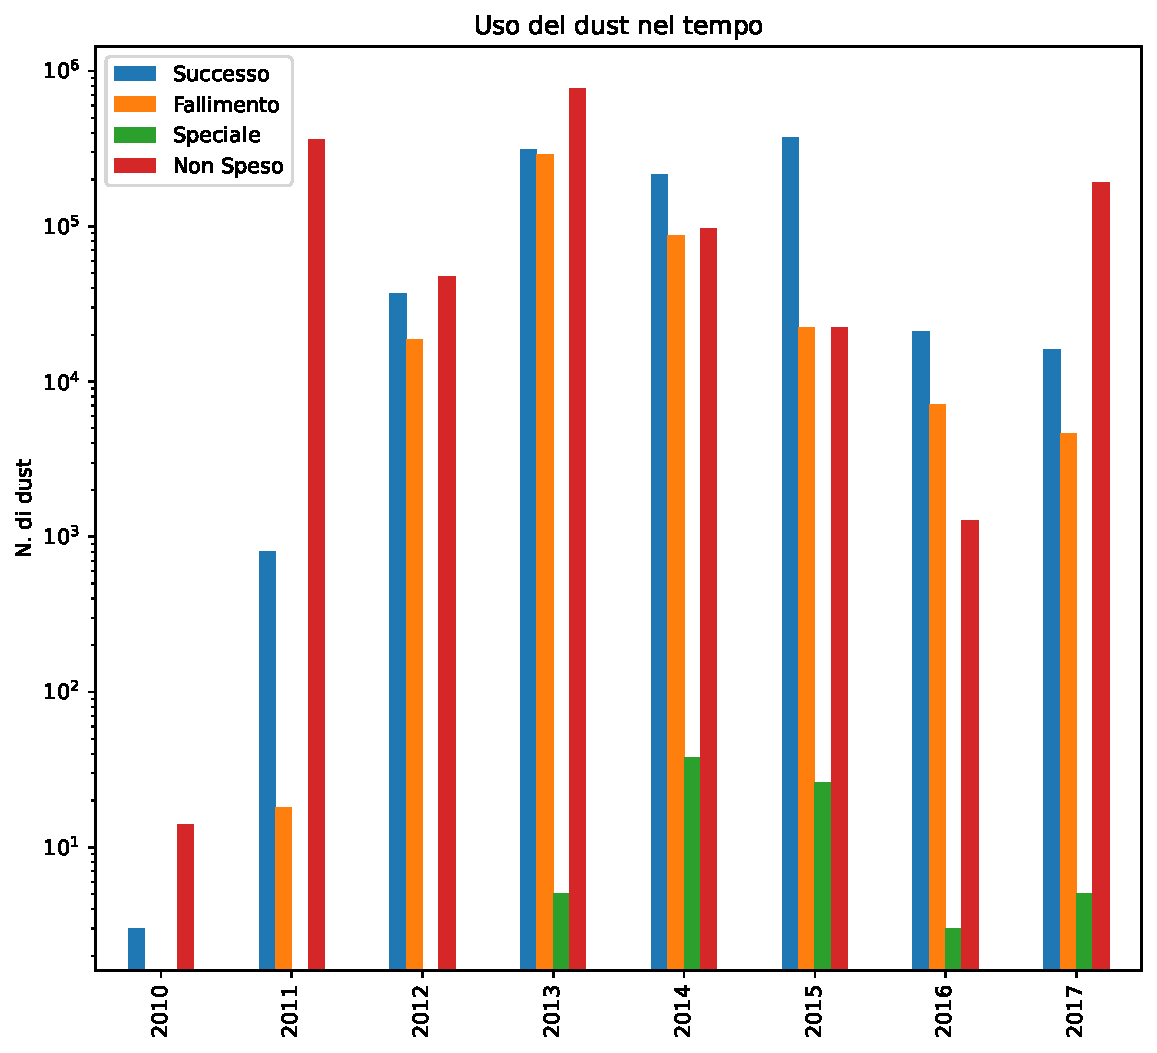
\includegraphics[scale=0.6]{Grafici/uso_del_dust_new.pdf}
    \caption{Uso finale (anche oltre l'anno di creazione considerato) degli output dust generati in un determinato anno}
    \label{fig:dust_year}
\end{figure}
\FloatBarrier

Non solo possiamo constatare graficamente quanto già detto in precedenza sulla differenza tra dust speso e non speso, ma possiamo anche fare due importanti riflessioni. 

La prima riflessione riguarda l'uso del servizio di ``dust collecting". Infatti risulta evidente quanto poco esso sia stato utilizzato. È importante notare che il dust della categoria ``Speciale" non necessariamente è legato a Dust-B-Gone, questa categoria infatti è presente anche nel 2017 nonostante il servizio sia stato ufficialmente chiuso nel 2016. Infatti rientrano in questa categoria anche gli utenti che decidono di propria iniziativa di spendere tutto il dust in fee. In generale non è possibile distinguere una transazione di ``dust-collecting" da una transazione generata da un singolo utente, tuttavia il numero di dust della categoria ``Speciale" permette di dare una sovrastima su quanto sia stato utilizzato questo servizio. Infatti il numero di dust spesi in transazioni di ``dust-collecting" può essere al massimo uguale al numero totale di dust della categoria ``Speciale".  

La seconda riflessione invece riguarda la tendenza a spendere il dust con almeno un altro address, in particolare notiamo un netto distacco nel 2015 dove la categoria ``Successo'' è nell’ordine di $10^4$ mentre ``Fallimento'' dell’ordine di $10^3$. In generale questa informazione è molto importante perché dimostra come il dust possa essere efficace per la de-anonimizzazione di un wallet, ovvero capire che più address appartengano ad un medesimo utente.

Una volta constatata la presenza di transazioni con input dust e con almeno due address diversi tra gli input, la fase seguente è l'analisi delle transazioni.

\section{Classificazione delle Transazioni}
Considereremo tre categorie di transazioni: 
\begin{itemize}
    \item \textbf{2+ address}: transazioni che presentano almeno due address di input differenti, la fee però è diversa dall'importo totale di input;
    \item \textbf{1 address}: transazioni con un singolo address di input;
    \item \textbf{speciale}: transazioni dove l'importo totale di input è uguale alla fee.
\end{itemize}

In totale il dust è stato speso in 263 963 transazioni, la tabella \ref{tab:tx_categories} mostra la percentuale delle transazioni nelle tre categorie, la tabella \ref{tab:tx_categories_year} mostra la distribuzione negli anni.
\begin{table}[H]
    \centering
    \begin{tabular}{|c|c|}
        \hline
        2+ address & 63,2\%\\
        \hline
        1 address & 36,7\%\\
        \hline
        speciale & 0,1\%\\
        \hline
    \end{tabular}
    \caption{Transazioni delle tre categorie}
    \label{tab:tx_categories}
\end{table}
\begin{table}[H]
    \centering
    \begin{tabular}{|l|c|c|c|c|c|c|c|c|}
        \hline
            categoria/anno  & 2010 & 2011 & 2012 & 2013 & 2014 & 2015 & 2016 & 2017\\
        \hline 
         2+ address(\%) & 100 & 93 & 55,6 & 68,4 & 55,9 & 64,5 & 62,7 & 75 \\
         \hline
         1 address(\%) & 0 & 7 & 44,4 & 31,5 & 44,09 & 35,4 & 37,2 & 24,7  \\
         \hline
         speciali(\%) & 0 & 0 & 0 & 0,1 & 0,01 & 0,1 & 0,1 & 0,3 \\
         \hline
    \end{tabular}
    \caption{Transazioni delle tre categorie nel tempo}
    \label{tab:tx_categories_year}
\end{table}
Dalle tabelle \ref{tab:tx_categories} \ref{tab:tx_categories_year} confermiamo quanto detto prima, la prevalenza a spendere il dust in transazioni con almeno due address diversi e lo scarso utilizzo di servizi come Dust-B-Gone. Siccome sono presenti solo 17 transazioni della terza categoria 
\subsection{Categoria 1 Address}
La categoria ``1 address" è stata ulteriormente suddivisa in due classi:
\begin{itemize}
    \item \textbf{NOD}(Not Only Dust): transazioni che presentanto almeno un input con importo maggiore di 545  
    \item \textbf{OD}(Only Dust): transazioni con soli input dust.
\end{itemize}

Dalla tabella \ref{tab:OD_NOD_failed} possiamo dedurre che il fallimento nella de-anonimizzazione sia dovuto principalmente a quegli address che presentano un saldo positivo, ovvero un bilancio complessivo maggiore di zero. In questo caso gli address hanno potuto spendere il dust con altri input provenienti tutti dal medesimo address, impedendo ad un possibile attaccante di creare un cluster da associare ad un unico utente.
\begin{table}[H]
    \centering
    \begin{tabular}{|c|c|c|}
        \hline
            NOD  & 92 712 & 95,5\%\\
        \hline 
            OD  & 4328 & 4,5 \%\\
        \hline
    \end{tabular}
    \caption{Classificazione OD e NOD}
    \label{tab:OD_NOD_failed}
\end{table}
Particolarmente interessante invece è il secondo gruppo, ed abbiamo approfondito manualmente in particolare due address appartenenti ad esso:
\begin{itemize}
    \item \textit{1JwSSubhmg6iPtRjtyqhUYYH7bZg3Lfy1T}
    \item \textit{1PEDJAibfNetJzM289oXsW1qLAgjYDjLgN}
\end{itemize}

Il fatto interessante del primo address è che la sua chiave privata è stata compromessa \footnote{fonte:\url{https://privatekeys.pw/address/bitcoin/1JwSSubhmg6iPtRjtyqhUYYH7bZg3Lfy1T}}, consentendo a chiunque di riscattare bitcoin non appena vengono inviati a questo address. Questo address è tipicamente destinatario di transazioni di 2936 output dust, con tutti gli importi destinati ad esso. Speigazione più probabile è che tale address venga utilizzato come metodo per scrivere dati arbitrari sulla blockchain (nascosti all'interno di pagamenti irrisori) minimizzando i costi.

Caso anomalo invece riguarda il secondo address, rinominato \textit{1PED} per semplicità. Questo address, come riportato in \cite{dustAnalisi}, sappiamo essere un noto gambler di Satoshi Dice, ma la sua singolarità deriva da alcune transazioni che ha generato. In queste transazioni infatti è presente un solo input di 1 satoshi e un solo output, ovviamente sempre di 1 satoshi. Questi singoli satoshi però non provengono da Satoshi Dice ma da altri address che seguono un pattern ben preciso, schematizzato nella figura \ref{fig:1PED}
\begin{figure}[h!]
    \centering
    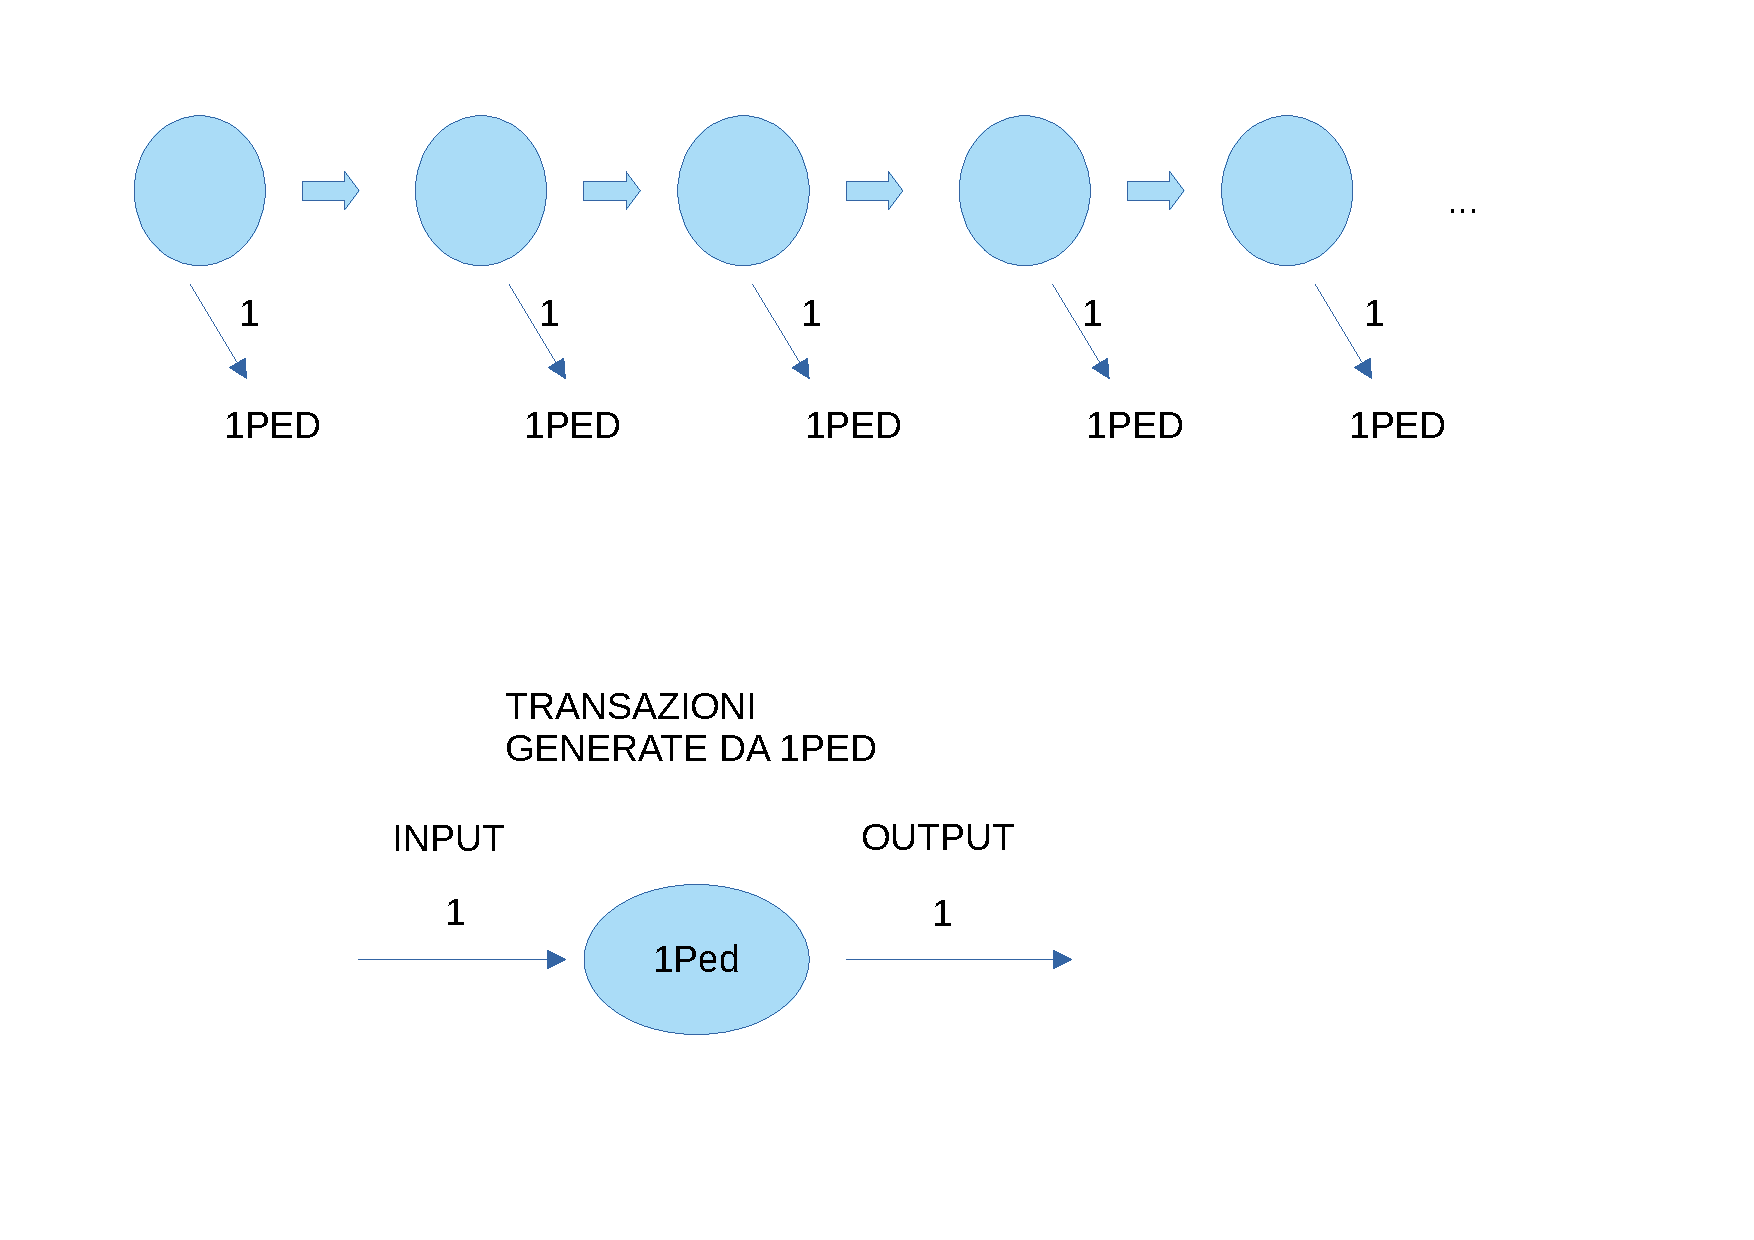
\includegraphics[scale=0.4]{Images/1Ped.pdf}
    \caption{Schema transazioni legate a \textit{1PED}}
    \label{fig:1PED}
\end{figure}
\FloatBarrier
Ogni address, appartenente al pattern, invia due output, 1 satoshi con destinatario \textit{1PED} e un secondo importo che viene inviato ad un altro address che seguirà il medesimo schema. In tutte queste transazioni la fee è sempre di 50 000 satoshi. \textit{1PED} ha generato poi 1835 transazioni con un solo satoshi di input ed un solo satoshi di output, tutte in data 10 Marzo 2013 alle ore 16:20. È interessante sottolineare come \textit{1PED} sia riuscito a spendere un singolo satoshi senza la necessità di aggregare il dust con altri input. Questo significa che, nonostante queste transazioni fossero non-standard, un miner ha comunque deciso di validarle, però sebbene questo comportamento sia anomalo risulta alquanto improbabile che si tratti di Dust Attack. Questa considerazione deriva dal fatto che tutti gli address di output delle transazioni generate da \textit{1PED} sono address mai comparsi prima nella blockchain.

\subsection{Categoria 2+ Address}
Una volta esaminate le transazioni ``1 address" il prossimo passaggio è l'analisi delle transazioni della categoria ``2+ address". Anche in questo caso vengono mostrati i gruppi OD e NOD. La tabella \ref{tab:OD_NOD_success} mostra come quasi sempre gli importi dust vengano aggregati ad altri importi non-dust.
\begin{table}[H]
    \centering
    \begin{tabular}{|c|c|c|}
        \hline
            NOD  & 166 778 & 99,9\%\\
        \hline 
            OD  & 128 & 0,1 \%\\
        \hline
    \end{tabular}
    \caption{Classificazione OD e NOD}
    \label{tab:OD_NOD_success}
\end{table}
è importante però capire quanto successo abbia avuto la deanonimizzazione causata dal dust, analizzando soprattutto gli address di input. In particolare è importante capire quanti address diversi ci siano all'interno di una singola transazione, in modo da capire il livello di de-anonimizzazione che il dust permette. Generalmente più address riesco ad unire in un singolo cluster, maggiore è il livello di de-anonimizzazione ottenuta, infatti più address associo ad un singolo utente maggiore è la tranciabilità dell'attività di quell'utente.

Il grafico \ref{fig:diff_addr} mostra la distribuzione del numero di address diversi. Osserviamo subito come un notevole numero di transazioni tende ad avere un numero di address nel primo intervallo, ovvero nell'intervallo [1, 50]. È possibile notare come sia presente un elevato numero di transazioni con centinaia di address di input. In tali transazioni è stato quindi possibile collegare centinaia di address diversi appartenenti ad un unico utente. Ad esempio la transazione con il maggior numero di address differenti contiene ben 1750 address diversi, nel qual caso è stato possibile collegare più di mille address ad un unico utente. In generale la media è di 13 address diversi per una singola transazione. 

 \begin{figure}[h!]
     \centering
     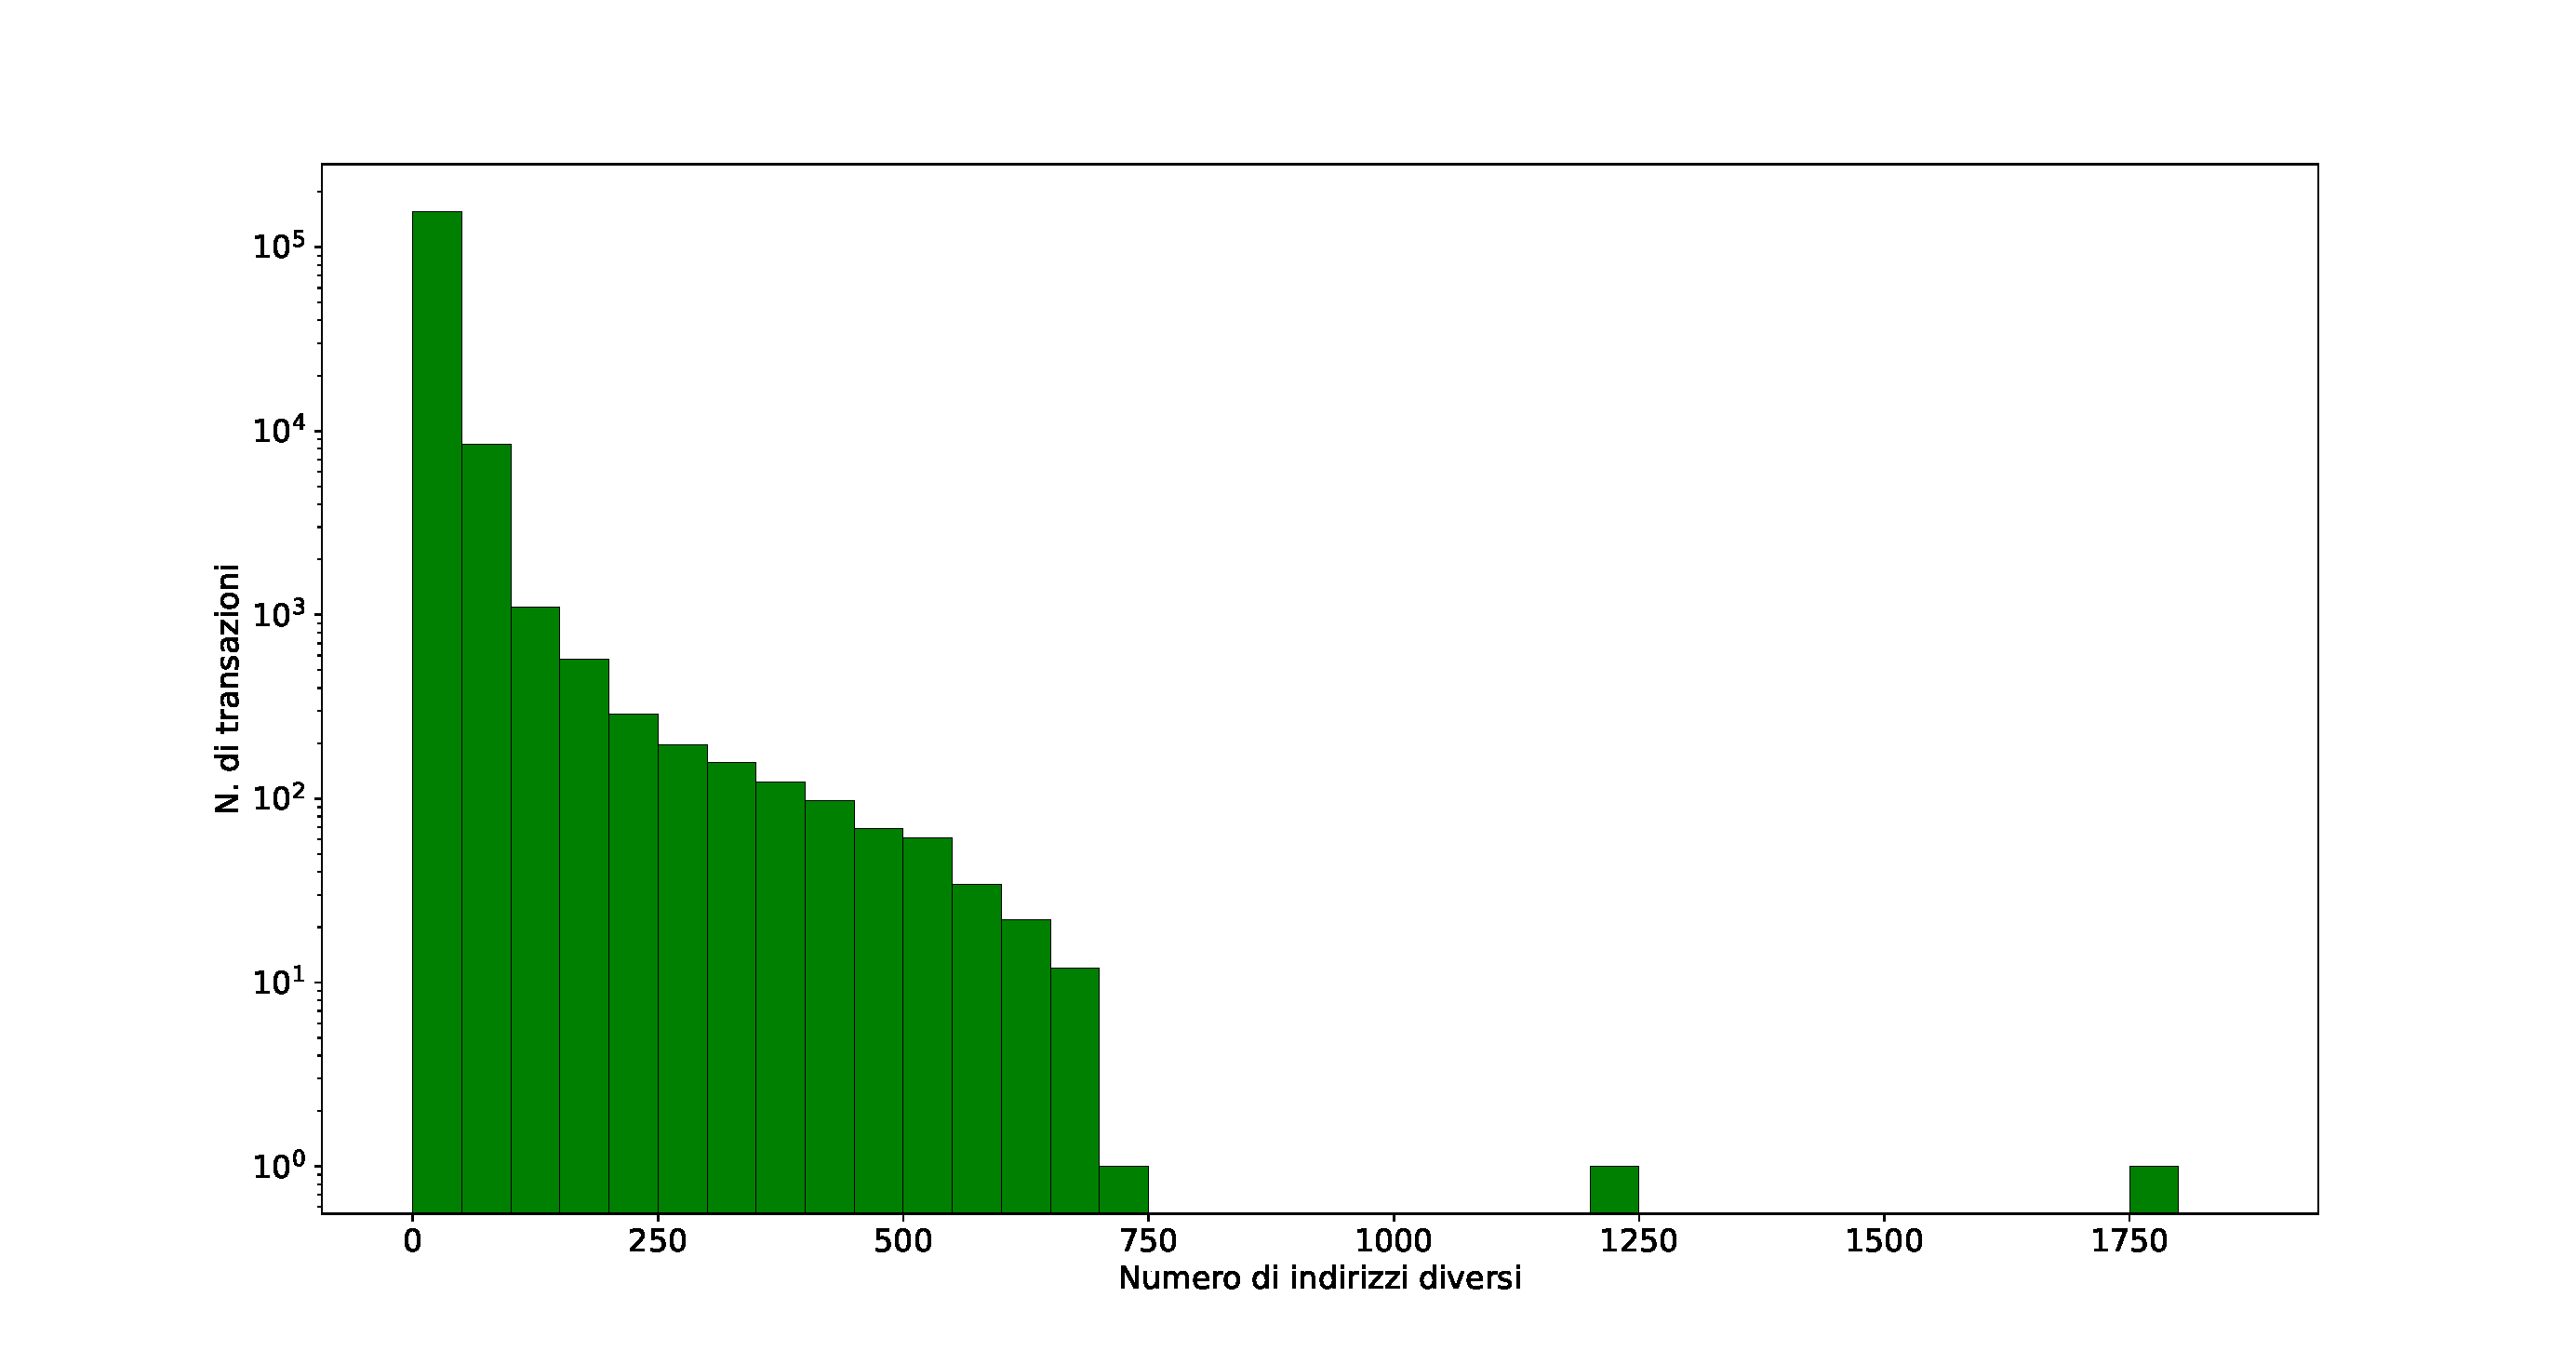
\includegraphics[scale=0.3]{Grafici/num_addr.pdf}
     \caption{Distribuzione numero address differenti. Colonne di ampiezza 50, la prima colonna rappresenta l'intervallo [1, 50] (anche se non possono esistere valori con un singolo address essendo nella categoria 2+ ``address'')}
     \label{fig:diff_addr}
 \end{figure}
\FloatBarrier
Questi dati sembrerebbero confermare l'efficacia del Dust Attack, tuttavia è importante precisare che stessi address possano apparire in più transazioni, quindi diverse transazioni potrebbero riferire i medesimi address di input, portando ad una de-anonimizzazione ripetuta. 

Nonostante siano stati generati 2 893 877 output dust gli address a cui sono stati inviati sono 1 059 836 e solo il 29\%(312 114) lo ha speso. Di questo 29\% abbiamo che 259 252 hanno speso il dust in transazioni della categoria ``2+ address" anche se 4 270 address hanno generato anche transazioni nella categoria ``1 address". Una particolarità interessante delle transazioni che hanno generato dust etichettato con ``Successo" è che in molti casi erano presenti tra gli output dust address nuovi, ovvero address che non erano mai comparsi sulla blockchain. 

Ci sono 98 198 transazioni che generano almeno un dust della categoria ``Successo", ma solo circa il 59\%(58 146) non presenta address nuovi tra gli output. Come spiegato in sezione \ref{dstatt} è molto improbabile che un attaccante invii del dust ad un address nuovo, perché risulterebbe strano de-anonimizzare un address mai visto. Nella fase finale della procedura di analisi, quindi, sono state considerate solo transazioni senza indirizzi nuovi, così da trovare dei pattern interessanti di possibili Dust Attack di successo. Nel paragrafo successivo verranno approfonditi due di tali possibili schemi di Dust Attack. 

\section{Analisi di Pattern Interessanti}\label{pattern}
In generale è complicato affermare con certezza se un address stia compiendo un Dust Attack, però abbiamo individuato due schemi, con certe proprietà, che rappresentano candidati sospetti di Dust Attack. La proprietà più importante riguarda l'assenza di address nuovi tra gli output dust, poichè è alquanto improbabile tentare di de-anonimizzare un address mai visto fino a quel punto.

Il primo pattern, sintetizzato in figura \ref{fig:schema1}, risulta molto simile al caso 1PED. Esistono diversi address legati a catena che generano transazioni con esattamente due output. Il secondo output, inviato sempre al solito address (probabilmente controllato dall'attaccante), viene speso dall'attaccante per generare transazioni contenenti solo output dust. Inoltre l'attaccante, nell'immagine l'ovale rosso, non compare mai nella catena dei finanziatori, rappresentata dai cerchi azzurri.
\begin{figure}[h!]
    \centering
    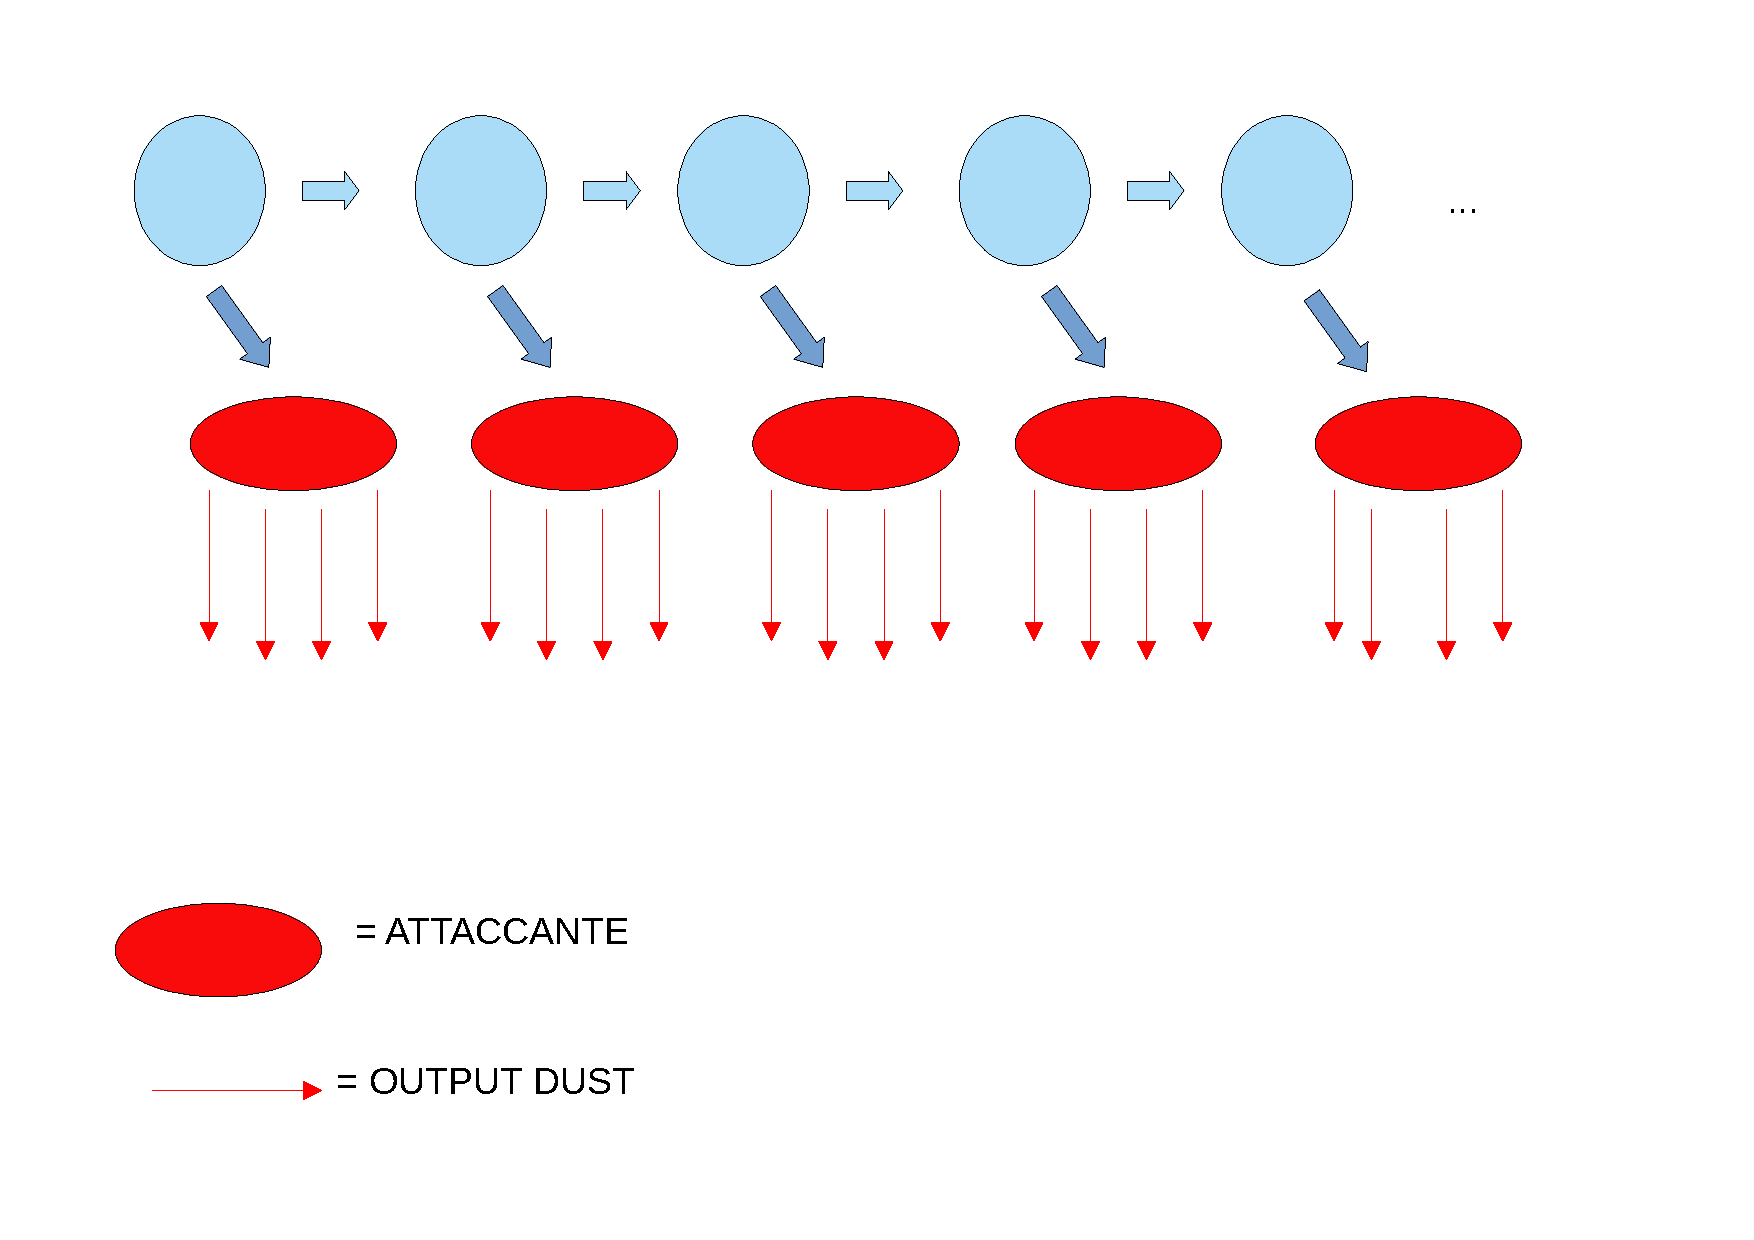
\includegraphics[scale=0.4]{Images/dust_attack1.pdf}
    \caption{Pattern ``Un finaziatore - un attaccante"}
    \label{fig:schema1}
\end{figure}
\FloatBarrier
Altre proprietà importanti di questo pattern sono: fare riferimento ad un unico finanziatore, generare sempre lo stesso numero di output dust, avere sempre il medesimo importo di input ed, infine, eseguire tutte le transazioni in un breve intervallo di tempo. Un esempio di tale schema è realizzato dall'address \textit{1DiRy9Giiq1GCkAD7VMSrXoKVe2dimnovm}, finanziato da \textit{1Nj3AsYfhHC4zVv1HHH4FzsYWeZSeVC8vj}. Inoltre sono presenti altri address che seguono lo stesso schema, pagati sempre dallo stesso finanziatore di $1DiRy$. Questo significa che il pattern appena enunciato può essere eseguito in parallelo utilizzando diversi address attaccanti.

Potrebbero esserci anche più finanziatori che inviano denaro a più attaccanti. Per esempio l'address \textit{16JLbXYe5xmxGNX8hiqooyTUJnhitNNqTh} ha ricevuto fondi da \textit{1NPfnbqZAMUnGuNuYwVZdCN4qVzUq4ejG4}, l'aspetto interessante però è che il numero di output dust, l'importo dust inviato, l'importo input speso sono esattamente uguali a quelli usati da \textit{1Diry}. Questo fatto fa ipotizzare che probabilmente questi address appartengano allo stesso utente o ad utenti con lo stesso obbiettivo. Ovviamente possono esserci eccezioni a questi due esempi trovati, per esempio avere più finanziatori o più attaccanti in una stessa catena. Inoltre gli importi e il numero di output dust potrebbero avere una natura più casuale. In generale si potrebbero ipotizzare diverse variazioni di questo pattern, anche se non ne abbiamo verificato la presenza.

Il secondo pattern riguarda le transazioni ``a catena" del 2013 citate nel paragrafo precedente. Questo schema è stato inizialmente scoperto tramite l'address \textit{1JYvvL67LrSGCG77cy4rmpUXCFfSub4JkG} (rinominato \textit{1JYvv}). Ogni address della catena invia centinaia o migliaia di output dust e il resto dell'importo viene inviato al prossimo address che seguirà lo stesso schema. La singolarità di questo modello è che gli address della catena, ad eccezione del primo, vengono utilizzati solo per eseguire quell'unica transazione. Non verranno mai più riutilizzati.
\begin{figure}[h!]
    \centering
    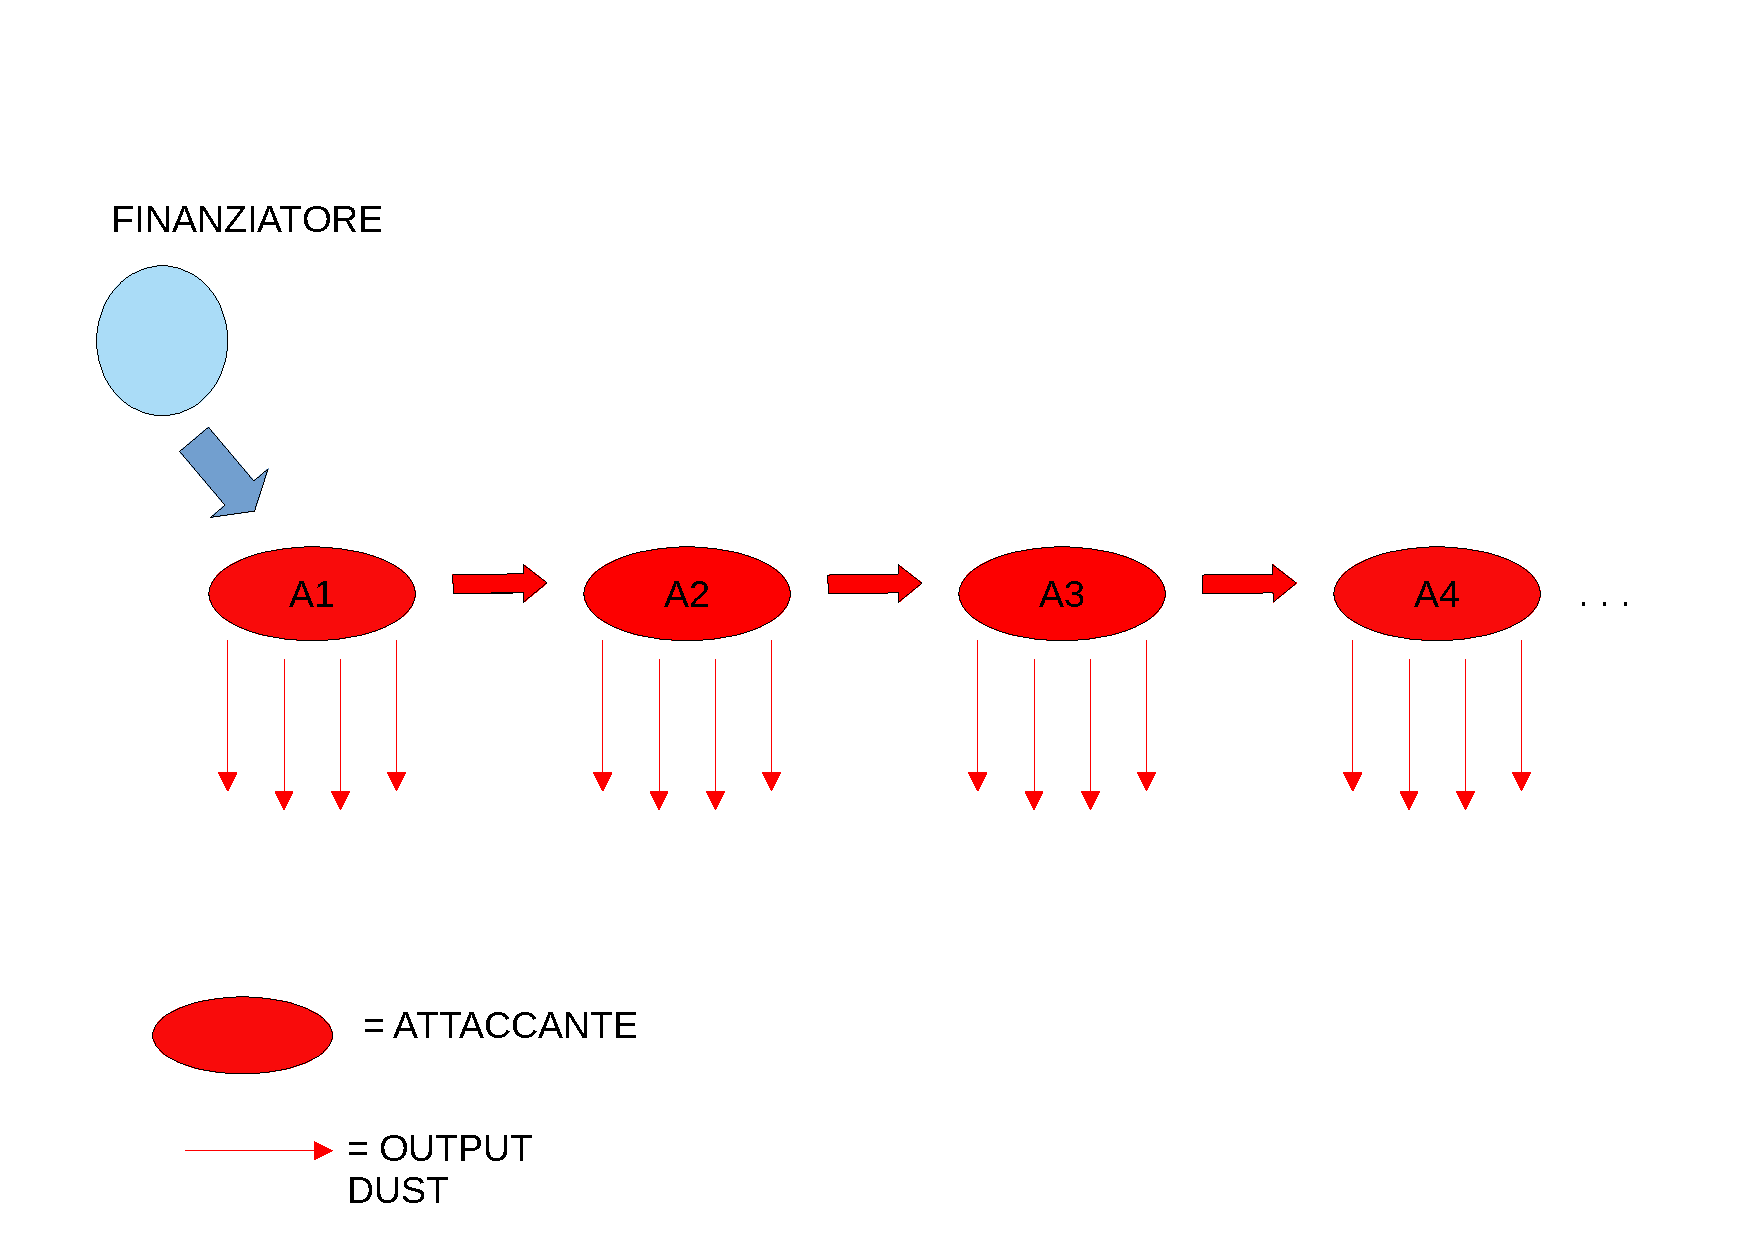
\includegraphics[scale=0.4]{Images/dust_attack2.pdf}
    \caption{Pattern ``Un finanziatore - più attaccanti"}
    \label{fig:schema2}
\end{figure}
\FloatBarrier
Consideriamo ad esempio l'address A3 della figura \ref{fig:schema2}. A3 riceve un importo da A2 che utilizza in parte per inviare centinaia o migliaia di output dust, ed il resto, esclusa la fee, viene inviato ad A4 che seguirà il medesimo schema. Gli address A2, A3 e A4 vengono utilizzati solo per eseguire queste transazioni, successivamente non verranno mai più riutilizzati, al contrario di A1 che viene usato per cominciare una serie di catene secondo questo schema.

Potrebbe essere interessante in futuro capire quanti address abbiano seguito schemi di questi tipo e se ci siano altri fini oltre a quello di un possibile Dust Attack.